\section{Joint-Space Tracking Results}

\subsection{Tracking Performance Metrics}
We evaluate control performance using three key metrics:
\begin{enumerate}
    \item RMS Tracking Error: $e_{\text{rms}} = \sqrt{\frac{1}{N} \sum_{k=1}^{N} (q_{\text{des}}[k] - q[k])^2}$
    \item Peak Absolute Error: $e_{\max} = \max_k |q_{\text{des}}[k] - q[k]|$  
    \item Disturbance Estimate RMS: $d_{\text{rms}} = \sqrt{\frac{1}{N} \sum_{k=1}^{N} \hat{d}[k]^2}$
\end{enumerate}

\subsection{Joint-Level Analysis}
\begin{table}[H]
    \centering
    \caption{Per-joint tracking performance (DOB observer)}
    \begin{tabular}{lccc}
        \toprule
        \textbf{Joint} & \textbf{RMS Error [rad]} & \textbf{Peak Error [rad]} & \textbf{RMS Est. [Nm]} \\
        \midrule
        J0 & 0.00272 & 0.00485 & 0.0488 \\
        J1 & 0.00822 & 0.13007 & 0.2162 \\
        J2 & 0.00767 & 0.12990 & 0.1756 \\
        J3 & 0.00261 & 0.00466 & 0.0117 \\
        J4 & 0.00564 & 0.12990 & 0.0606 \\
        J5 & 0.00565 & 0.12990 & 0.0098 \\
        \midrule
        \textbf{Mean} & \textbf{0.00575} & \textbf{0.09321} & \textbf{0.0988} \\
        \bottomrule
    \end{tabular}
\end{table}

Excellent tracking on proximal joints (J0, J3) with RMS errors below 3 mrad. Moderate errors on intermediate joints reflect higher friction and payload effects. Disturbance magnitudes correlate with observed friction characteristics.

\subsection{Time-Domain Analysis}
Fig.\ref{fig:joint_0_time} shows Joint 0 tracking over 28.87 seconds. The actual position (red) closely follows the desired trajectory (green) with minimal steady-state error. Control torque ripples reflect friction and sensor noise, while the disturbance estimate captures unmodeled dynamics.

\begin{figure}[H]
    \centering
    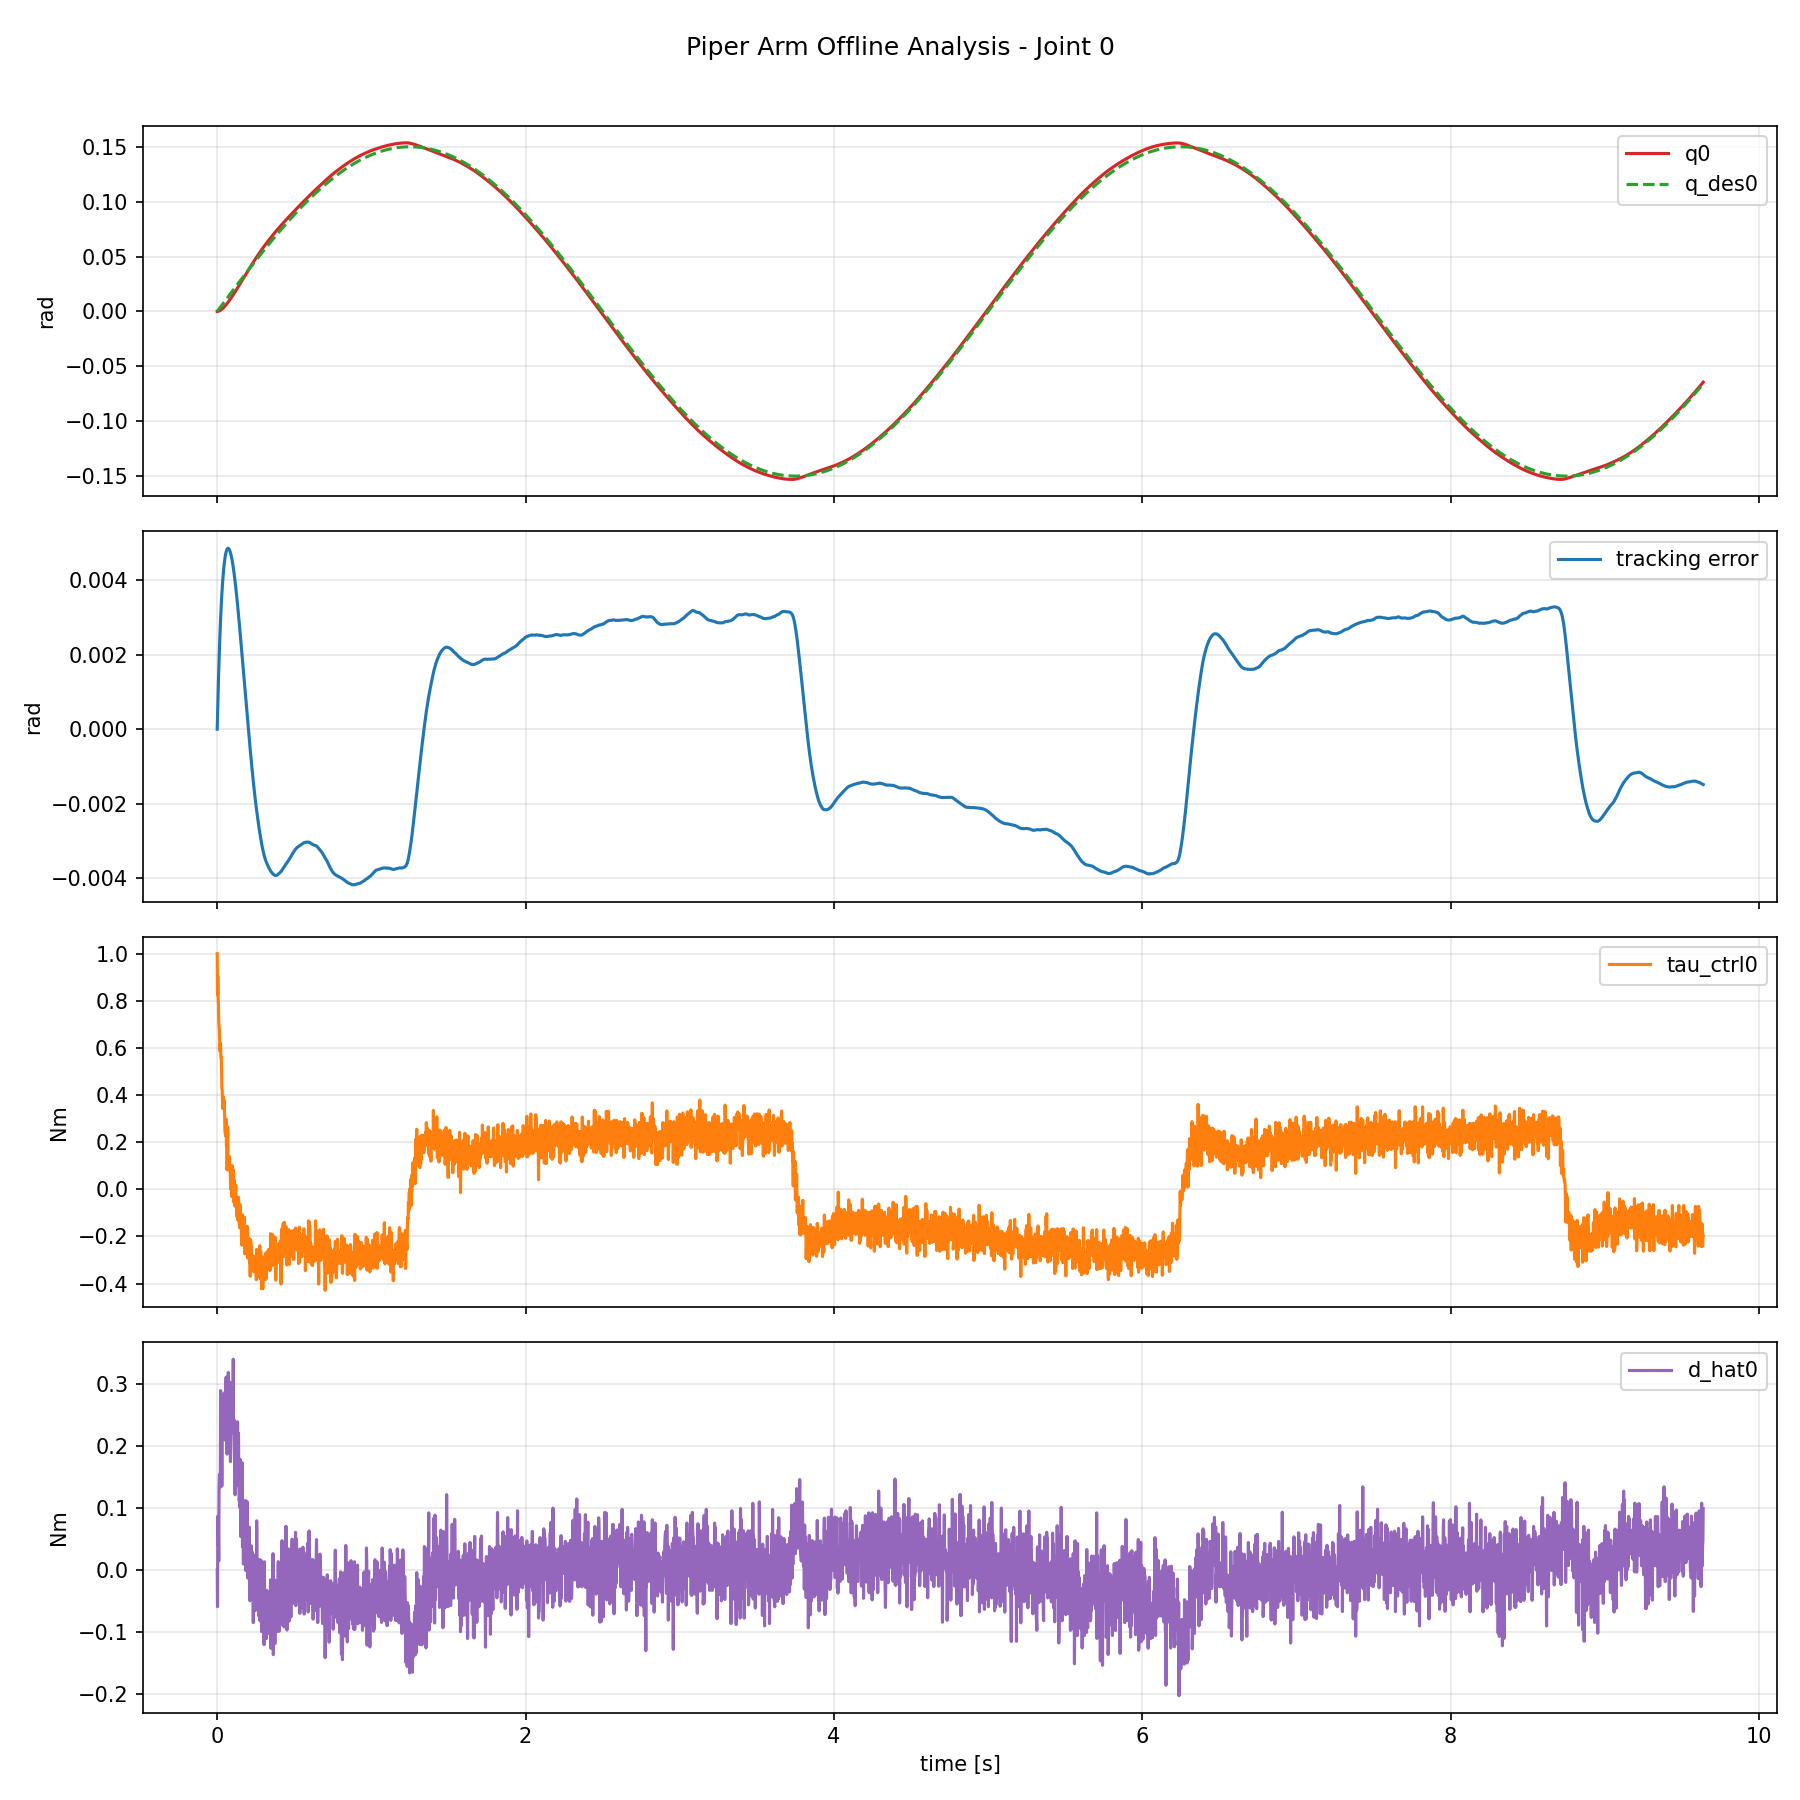
\includegraphics[width=0.9\textwidth]{figures/joint_0_analysis.png}
    \caption{Joint 0 time-domain analysis showing excellent position tracking, small error bounds, and low disturbance estimates.}
    \label{fig:joint_0_time}
\end{figure}

\subsection{Phase Plane Results}
Fig.\ref{fig:joint_0_phase} presents the phase portrait for Joint 0, with actual position versus desired position. The tight clustering around the diagonal $q = q_{\text{des}}$ indicates near-perfect tracking throughout the reference trajectory.

\begin{figure}[H]
    \centering
    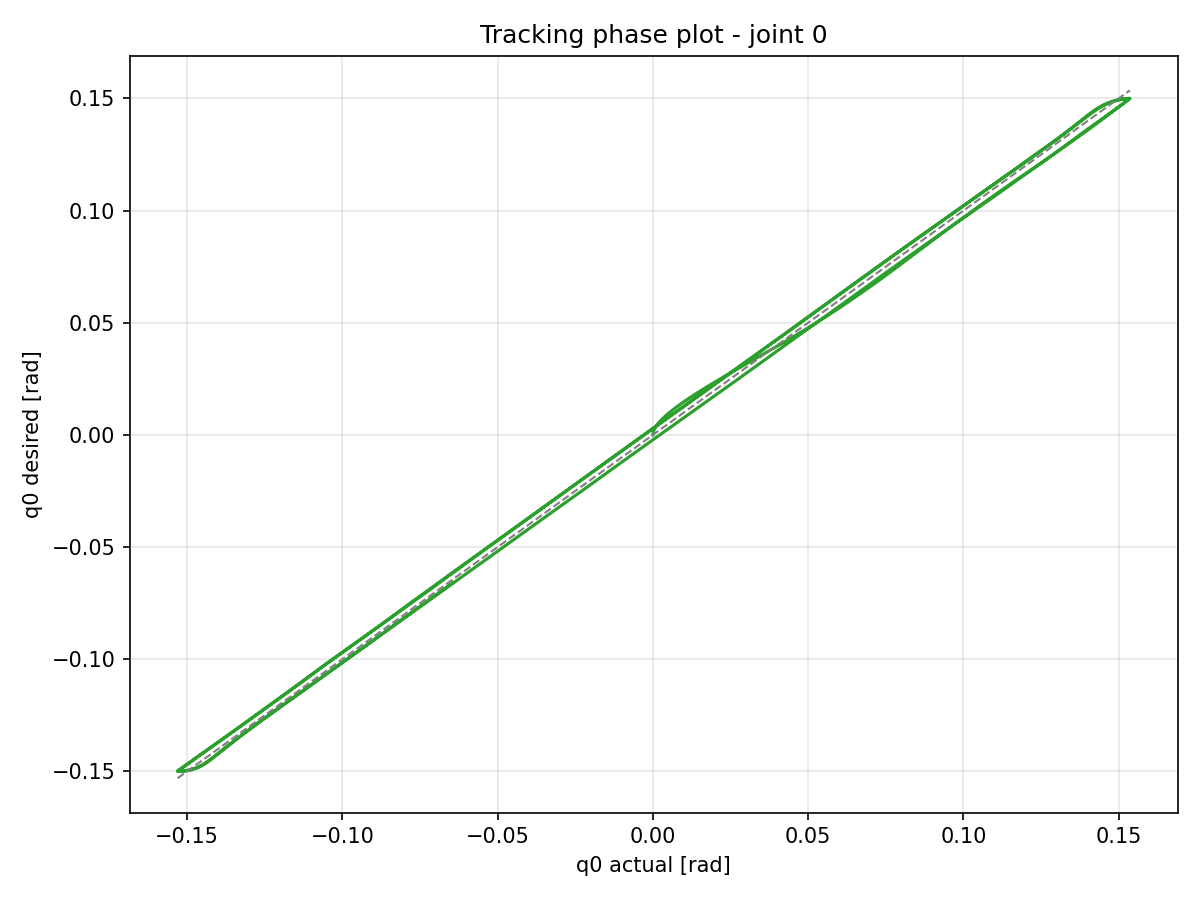
\includegraphics[width=0.7\textwidth]{figures/joint_0_phase.png}
    \caption{Phase portrait: Joint 0 actual vs. desired shows near-zero steady-state error across the full trajectory range.}
    \label{fig:joint_0_phase}
\end{figure}
